
\section{Overview}
\label{sec:overview}

This section illustrates \name with an encoding of a family polymorphism
solution to the Expression Problem, and informally presents its salient
features.

%-------------------------------------------------------------------------------
\subsection{Motivation: Family Polymorphism}

In OOP \emph{family polymorphism} is the ability to
simultaneously refine a family of related classes through inheritance. This is
motivated by a need to not only refine individual classes, but also to preserve
and refine their mutual relationships. Nystrom et al.~\cite{Nystrom_2004} call this
\emph{scalable extensibility}: ``the ability to extend a body of code while
writing new code proportional to the differences in functionality''.
%
A well-studied mechanism to achieve family inheritance is \emph{nested
inheritance}~\cite{Nystrom_2004}. Nested inheritance combines two aspects.
Firstly, a class can have nested class members; the outer class is then a
family of (inner) classes. Secondly, when one family extends another, it
inherits (and can override) all the class members, as well as the relationships
within the family (including subtyping) between the class members. However,
the members of the new family do not become subtypes of those in the parent family.

\paragraph{The Expression Problem, Scandinavian Style.}
Ernst~\cite{Ernst_2001} illustrates the benefits of nested inheritance for modularity
and extensibility with one of the most elegant and concise solutions to the
\emph{Expression Problem}~\cite{wadler1998expression}. The objective of the
Expression Problem is to extend a datatype, consisting of several cases,
together with several associated operations in two dimensions: by adding more
cases to the datatype and by adding new operations for the datatype.
Ernst solves the Expression Problem in the gbeta language,
which he adorns with a Java-like syntax for presentation purposes, for a small
abstract syntax tree (AST) example. His starting point is the code shown in
\cref{fig:lang}. The outer class \lstinline{Lang} contains a family of related
AST classes: the common superclass \lstinline{Exp} and two cases,
\lstinline{Lit} for literals and \lstinline{Add} for addition. The AST comes
equipped with one operation, \lstinline{toString}, which is implemented by both
cases.


\begin{figure}[t]
    \centering
    \begin{subfigure}[b]{0.45\textwidth}
\begin{lstlisting}[language=gbeta]
class Lang {
  virtual class Exp {
    String toString() {}
  }
  virtual class Lit extends Exp {
    int value;
    Lit(int value) {
      this.value = value;
    }
    String toString() {
      return value;
    }
  }
  virtual class Add extends Exp {
    Exp left,right;
    Add(Exp left, Exp right) {
      this.left = left;
      this.right = right;
    }
    String toString() {
      return left + "+" + right;
    }
  }
}
\end{lstlisting}
\subcaption{Base family: the language \lstinline{Lang}} \label{fig:lang}
    \end{subfigure} ~
    \begin{subfigure}[b]{0.5\textwidth}
\begin{lstlisting}[language=gbeta,  xleftmargin=1mm]
// Adding a new operation
class LangEval extends Lang {
  refine class Exp {
    int eval() {}
  }
  refine class Lit {
    int eval { return value; }
  }
  refine class Add {
    int eval { return
      left.eval() + right.eval();
    }
  }
}
// Adding a new case
class LangNeg extends Lang {
  virtual class Neg extends Exp {
    Neg(Exp exp) { this.exp = exp; }
    String toString() {
      return "-(" + exp + ")";
    }
    Exp exp;
  }
}
\end{lstlisting}
\subcaption{Extending in two dimensions} \label{fig:extend}
    \end{subfigure}
    \caption{The Expression Problem, Scandinavian Style}
\end{figure}

\paragraph{Adding a New Operation.}
One way to extend the family is to add an additional evaluation operation, as
shown in the top half of \cref{fig:extend}. This is done by subclassing the
\lstinline{Lang} class and refining all the contained classes by implementing
the additional \lstinline{eval} method. Note that the inheritance between, e.g.,
\lstinline{Lang.Exp} and \lstinline{Lang.Lit} is transferred to
\lstinline{LangEval.Exp} and \lstinline{LangEval.Lit}. Similarly, the
\lstinline{Lang.Exp} type of the \lstinline{left} and \lstinline{right} fields
in \lstinline{Lang.Add} is automatically refined to \lstinline{LangEval.Exp} in
\lstinline{LangEval.Add}.

\paragraph{Adding a New Case.}
A second dimension to extend the family is to add a case for negation, shown in
the bottom half of \cref{fig:extend}. This is similarly achieved by subclassing
\lstinline{Lang}, and now adding a new contained class \lstinline{Neg}, for
negation, that implements the \lstinline{toString} operation.

Finally, the two extensions are naturally combined by means of
multiple inheritance, closing the diamond.
\begin{lstlisting}[language=gbeta]
class LangNegEval extends LangEval & LangNeg {
  refine class Neg {
    int eval() { return -exp.eval(); }
  }
}
\end{lstlisting}
The only effort required is to implement the one missing operation
case, evaluation of negated expressions.

% \paragraph{A solution in \name using nested composition:} Show a
% solution in \name with records implemented in SEDEL. Justify the connection to the
% class-based solution. Mention that type system support
% for family polymorphism is known to be hard.

%-------------------------------------------------------------------------------
\subsection{The Expression Problem, \name Style}

The \name calculus allows us to solve the Expression Problem in a way that is
very similar to Ernst's gbeta solution. However, the underlying mechanisms of
\name are quite different from those of gbeta. In particular, \name features a
structural type system in which we can model objects with records, and object
types with record types. For instance, we model the interface of \lstinline{Lang.Exp}
with the singleton record type \lstinline${ print : String }$. For the sake of
conciseness, we use type aliases to abbreviate types.
\lstinputlisting[linerange=4-4]{./examples/overview.sl}% APPLY:linerange=PRINT_INTERFACE
Similarly, we capture the interface of the \lstinline{Lang} family in a record,
with one field for each case's constructor.
\lstinputlisting[linerange=8-8]{./examples/overview.sl}% APPLY:linerange=LANG_FAMILY
Here is the implementation of \lstinline{Lang}.
\lstinputlisting[linerange=17-22]{./examples/overview.sl}% APPLY:linerange=LANG_IMPL

% - - - - - - - - - - - - - - - - - - - - - - - - - - - - - - - - - - - - - - - -
\paragraph{Adding Evaluation.}
We obtain \lstinline{IPrint & IEval}, which is the corresponding type for \lstinline{LangEval.Exp}, by
intersecting \lstinline{IPrint} with \lstinline{IEval} where
\lstinputlisting[linerange=27-27]{./examples/overview.sl}% APPLY:linerange=EVAL_INTERFACE
The type for \lstinline{LangEval} is then:
\lstinputlisting[linerange=32-35]{./examples/overview.sl}% APPLY:linerange=EVAL_PRINT_INTERFACE
We obtain an implementation for \lstinline{LangEval} by merging the existing
\lstinline{Lang} implementation \lstinline{implLang} with the new evaluation
functionality \lstinline{implEval} using the merge operator \lstinline{,,}.
\lstinputlisting[linerange=43-49]{./examples/overview.sl}% APPLY:linerange=EVAL_PRINT_IMPL

% - - - - - - - - - - - - - - - - - - - - - - - - - - - - - - - - - - - - - - - -
\paragraph{Adding Negation.}
Adding negation to \lstinline{Lang} works similarly.
\lstinputlisting[linerange=53-59]{./examples/overview.sl}% APPLY:linerange=LANG_NEG
% \begin{Verbatim}[xleftmargin=10mm,fontsize=\relscale{.80}]
% type LangNeg = Lang & { neg : IPrint -> IPrint }

% implLangNeg : LangNeg
% implLangNeg = implLang ,, implNeg

% implNeg = { neg = \a.{print = "-" ++ a.print } }
% \end{Verbatim}

% - - - - - - - - - - - - - - - - - - - - - - - - - - - - - - - - - - - - - - - -
\paragraph{Putting Everything Together.}
Finally, we can combine the two extensions and provide the missing
implementation of evaluation for the negation case.
\lstinputlisting[linerange=64-71]{./examples/overview.sl}% APPLY:linerange=LANG_FINAL
We can test \lstinline{implLangNegEval} by creating an object \lstinline{e} of expression $-2 + 3$ that is able to print and evaluate at the same time.
\lstinputlisting[linerange=89-91]{./examples/overview.sl}% APPLY:linerange=TEST



%- - - - - - - - - - - - - - - - - - - - - - - - - - - - - - - - - - - - - - - -
\paragraph{Multi-Field Records.} One relevant remark is that
\name does not have multi-field record types built in. They are merely syntactic
sugar for intersections of single-field record types. Hence, the following is an
equivalent definition of \lstinline{Lang}:
\lstinputlisting[linerange=13-13]{./examples/overview.sl}% APPLY:linerange=LANG_FAMILY2
Similarly, the multi-field record expression in the definition of
\lstinline{implLang} is syntactic sugar for the explicit merge of two
single-field records.
\begin{lstlisting}
implLang : Lang = { lit = ... } ,, { add = ... };
\end{lstlisting}

%- - - - - - - - - - - - - - - - - - - - - - - - - - - - - - - - - - - - - - - -
\paragraph{Subtyping.}
A big difference compared to gbeta is that many more \name types are related through
subtyping. Indeed, gbeta is unnecessarily conservative~\cite{ernst_hoh}: none of the families is related
through subtyping, nor is any of the class members of one family related to any
of the class members in another family. For instance, \lstinline{LangEval} is
not a subtype of \lstinline{Lang}, nor is \lstinline{LangNeg.Lit} a subtype
of \lstinline{Lang.Lit}.

In contrast, subtyping in \name is much more nuanced and depends entirely on the
structure of types. The primary source of subtyping are intersection types:
any intersection type is a subtype of its components. For instance, 
\lstinline{IPrint & IEval} is a subtype of both \lstinline{IPrint} and
\lstinline{IEval}. Similarly \lstinline{LangNeg = Lang & NegPrint} is a subtype
of \lstinline{Lang}. Compare this to gbeta where \lstinline{LangEval.Expr} is
not a subtype of \lstinline{Lang.Expr}, nor is the family \lstinline{LangNeg} a
subtype of the family \lstinline{Lang}.

However, gbeta and \name agree that \lstinline{LangEval} is not a subtype of
\lstinline{Lang}. The \name-side of this may seem contradictory at first, as we
have seen that intersection types arise from the use of the merge operator, and
we have created an implementation for \lstinline{LangEval} with
\lstinline{implLang ,, implEval} where \lstinline{implLang : Lang}. That
suggests that \lstinline{LangEval} is a subtype of \lstinline{Lang}.
Yet, there is a flaw in our reasoning:
strictly speaking, \lstinline{implLang ,, implEval} is not of
type \lstinline{LangEval} but instead of type \lstinline{Lang & EvalExt}, where
\lstinline{EvalExt} is the type of \lstinline{implEval}:
\lstinputlisting[linerange=39-39]{./examples/overview.sl}% APPLY:linerange=EVAL_INTERFACE2
Nevertheless, the definition of \lstinline{implLangEval} is valid because
\lstinline{Lang & EvalExt} is a subtype of \lstinline{LangEval}.
Indeed, if we consider for the sake of simplicity only the \lstinline{lit}
field, we have that \lstinline{(Int -> IPrint) & (Int -> IEval)} is a
subtype of \lstinline{Int -> IPrint & IEval}. This follows from a standard
subtyping axiom for distributivity of functions and intersections in the BCD system inherited by \name.
In conclusion, \lstinline{Lang & EvalExt} is a subtype of both \lstinline{Lang}
and of \lstinline{LangEval}. However, neither of the latter two types is a subtype of the other.
Indeed, \lstinline{LangEval} is not a subtype of \lstinline{Lang} as the type
of \lstinline{add} is not covariantly refined and thus admitting the subtyping
is unsound. For the same reason \lstinline{Lang} is not a subtype of \lstinline{LangEval}.


\Cref{fig:diagram} shows the various relationships between the language
components. Admittedly, the figure looks quite complex because our calculus
features a structural type system (as often more foundational calculi do),
whereas mainstream OO languages have nominal type systems. This is part of the
reason why we have so many subtyping relations in \cref{fig:diagram}.

\begin{figure}[t]
  \centering
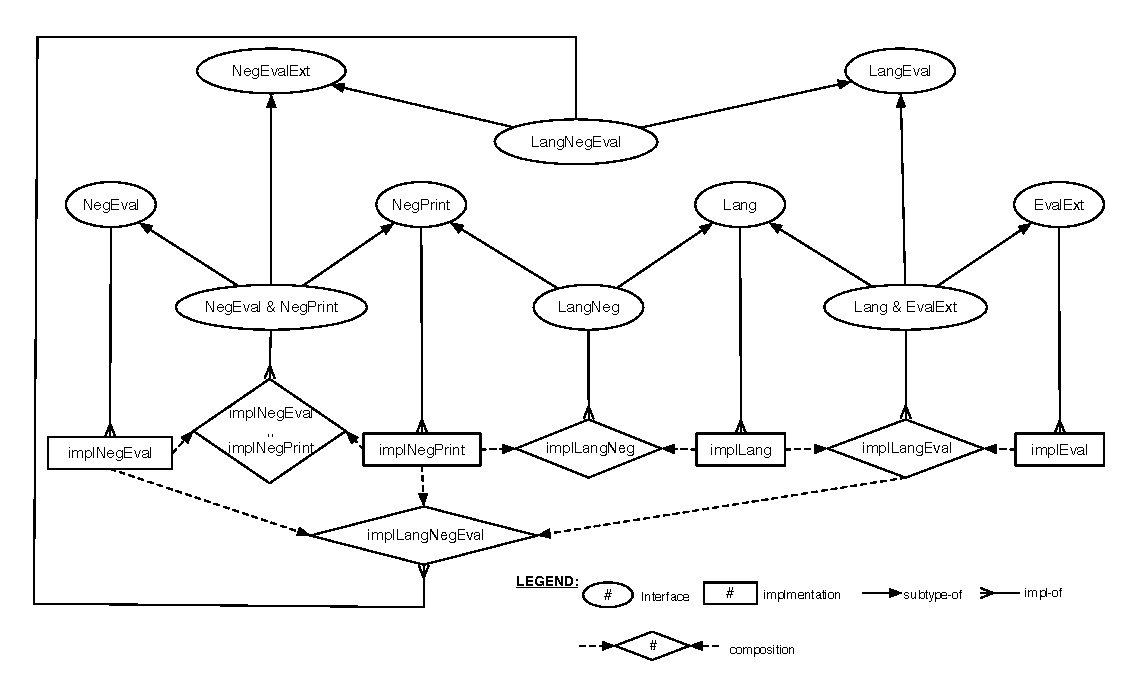
\includegraphics[scale=0.75]{diagram.eps}
\caption{Summary diagram of the relationships between language components}
\label{fig:diagram}
\end{figure}


\paragraph{Stand-Alone Extensions.}
Unlike in gbeta and other class-based inheritance systems, in \name
the extension \lstinline{implEval} is not tied to \lstinline{LangEval}. In that
sense, it resembles trait and mixin systems that can apply the same extension
to different classes. However, unlike those systems, \lstinline{implEval} can also
exist as a value on its own, i.e., it is not an extension per se.

%-------------------------------------------------------------------------------
\subsection{Disjoint Intersection Types and Ambiguity}

The above example shows that intersection types and the merge operator
are closely related to multiple
inheritance. Indeed, they share a major concern with multiple inheritance,
namely ambiguity. When a subclass inherits an implementation of the same
method from two different parent classes, it is unclear which of the two
methods is to be adopted by the subclass. In the case where the two parent classes
have a common superclass, this is known as the \emph{diamond problem}.
The ambiguity problem also appears in \name,
e.g., if we merge two numbers to obtain $\mer{1}{2}$ of type
$\inter{\mathsf{Nat}}{\mathsf{Nat}}$. Is the result of $\mer{1}{2} + 3$
either $4$ or $5$?

Disjoint intersection types offer to statically detect potential ambiguity and
to ask the programmer to explicitly resolve the ambiguity by rejecting the
program in its ambiguous form. In the previous work on \oname, ambiguity is
avoided by dictating that all intersection types have to be disjoint, i.e.,
$\inter{\mathsf{Nat}}{\mathsf{Nat}}$ is ill-formed because the first component
has the same type as the second.

\paragraph{Duplication is Harmless.}
While requiring that all intersections are disjoint is sufficient to guarantee
coherence, it is not necessary. In fact,
such requirement unnecessarily encumbers the subtyping definition with disjointness constraints
and an ad-hoc treatment of ``top-like'' types. Indeed, the value $\mer{1}{1}$
of the non-disjoint type $\inter{\mathsf{Nat}}{\mathsf{Nat}}$ is entirely unambiguous, and
$(\mer{1}{1}) + 3$ can obviously only result in $4$. More generally, when the
overlapping components of an intersection type have the same value, there is no
ambiguity problem. \name uses this idea to relax \oname's enforcement of
disjointness. In the case of a merge, it is hard to statically decide whether
the two arguments have the same value, and thus \name still requires
disjointness. This is why in \cref{fig:diagram} we cannot define
\lstinline{implLangNegEval} by directly composing the two existing
\lstinline{implLangEval} and \lstinline{implLangNeg}, even though the latter two
both contain the same \lstinline{implLang}.
Yet, disjointness is no longer required for the well-formedness
of types and overlapping intersections can be created implicitly through
subtyping, which results in duplicating values at runtime. For instance, while
$\mer{1}{1}$ is not expressible
$ 1 : \inter{\mathsf{Nat}}{\mathsf{Nat}}$ creates the equivalent value implicitly.
% The consequence of this relaxation of disjointness is a much simplified
% type system for \name.
In short, duplication is harmless and subtyping only generates duplicated
values for non-disjoint types.

% Disjoint intersection types ensure unambiguity and conflicts are
% statically detected and manually resolved by programmers. This
% is similar to the trait model.

%-------------------------------------------------------------------------------
\subsection{Logical Relations for Coherence}

Coherence is easy to establish for \oname as its rigid rules mean that there is
at most one possible subtyping derivation between any two types.  As a
consequence there is only one possible elaboration and thus one
possible behavior for any program.

Two factors make establishing coherence for \name much more difficult: the
relaxation of disjointness and the adoption of the more expressive subtyping
rules from the BCD system (for which \oname lacks). These two factors mean that subtyping proofs are no
longer unique and hence that there are multiple elaborations of the same source
program. For instance, $\inter{\mathsf{Nat}}{\mathsf{Nat}}$ is a subtype of $\mathsf{Nat}$ in two
ways: by projection on either the first or second component.
Hence the fact that all elaborations yield the same result when evaluated has
become a much more subtle property that requires sophisticated reasoning.
For instance, in the example, we can see that coherence holds because  at
runtime any value of type $\inter{\mathsf{Nat}}{\mathsf{Nat}}$ has identical components, and
thus both projections yield the same result.

For \name in general, we show coherence by capturing the non-ambiguity
invariant in a logical relation and showing that it is preserved by the
operational semantics. A complicating factor is that not one, but two languages
are involved: the source language \name and the target language, essentially
the simply-typed lambda calculus extended with coercions and records. The
logical relation does not hold for target programs and program contexts in
general, but only for those that are the image of a corresponding source
program or program context. Thus we must view everything through the lens of
elaboration.

% Local Variables:
% TeX-master: "../paper"
% org-ref-default-bibliography: ../paper.bib
% End:
